\section{Basic concepts}
\subsection{basic data structure (StreamNet)}
StreamNet is the underlying data structure in DAG. It is a Directed Acyclic Graph, where each node in the DAG represents a transaction and the directed edge represents a confirmation relationship between transactions. For example, site 0 in Figure 1 represents the Genesis transaction, which is initially identifiable as a confirmed transaction (in theory, it is also a 100\%confirmed transaction). Site1, on the other hand, represents the first transaction, which is confirmed by the subsequent site 2, 3, 4. When a new transaction is not confirmed, it is called a tip. For example, in Figure 1, site 6 is a tip.


\begin{figure}[H]
	\centering
	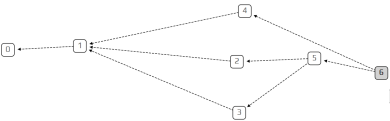
\includegraphics[width=3.0in]{figures/screenshot001.png}
	\caption{DAG shows [1]}
	\label{simulationfigure}
\end{figure}

\subsection{Trading}
\subsubsection{Creation Trading}
There is no concept of mining in StreamNet, and all tokens are included in the creation transaction block. In Figure 2, a creation transaction is described with an initial token number of 5.

\begin{figure}[H]
	\centering
	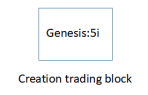
\includegraphics[width=2.0in]{figures/screenshot002.png}
	\caption{Genesis Block}
	\label{simulationfigure}
\end{figure}

\subsubsection{Trading Content}
Assume that in Figure 2, Genesis wants to transfer 1 token to Alice, and then hopes to transfer 1 token to Bob and attach the transaction block corresponding to this transfer to StreamNet, then the resulting StreamNet is shown in Figure 3. Here, each transaction must find two tip transactions to confirm, namely trunk and branch transactions. For example, Genesis $\rightarrow$ Alice's transaction confirms the Genesis transaction itself, while Genesis $\rightarrow$ Bob's transaction confirms the Genesis transaction itself and Genesis $\rightarrow$ Alice's transaction. When a transaction wants to be attached to StreamNet, it must do enough Workload Proof (POW) [2], but this POW differs from Bitcoin in that its difficulty is fixed and therefore does not need to be The participation of miners [3].

\begin{figure}[H]
	\centering
	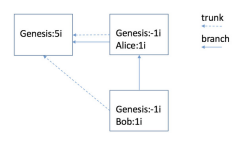
\includegraphics[width=3.0in]{figures/screenshot003.png}
	\caption{shows the transfer transaction}
	\label{simulationfigure}
\end{figure}

\subsubsection{transaction verification (approve)}
Because a new transaction needs to find two tip transactions for approval, the verification method has two steps:
\begin{itemize}
\item with Genesis, verify all transactions that are directly or indirectly referenced, mainly to see if this will result in a negative balance or loss of the token [1]. For example, in Figure 4, Alice $\rightarrow$ Sam's transfer needs to verify transactions that are indirectly or directly referenced. Then it constructs a topological sequence according to the characteristics of DAG, namely (Genesis) $\rightarrow$ (Genesis $\rightarrow$ Alice) $\rightarrow$ (Genesis $\rightarrow$ Bob) $\rightarrow$ (Alice $\rightarrow$ Sam), and finds that each step does not violate the principle of transfer. Then the verification is successful. In Figure 5, the same topology sequence, when verifying (Genesis $\rightarrow$ Bob), because the Genesis balance will be reduced to -1, the verification fails, as an honest node, Alice $\rightarrow$ Sam transaction Will find a new tip to verify, but it can also choose to spoof, attach this transaction to the selected tip. However, such an approach is likely to result in subsequent rejection of its own transactions.
\item At the same time, the signature needs to be checked during the verification of the topology sequence to ensure that the link relationship has not been tampered with.
\end{itemize}

\begin{figure}[H]
	\centering
	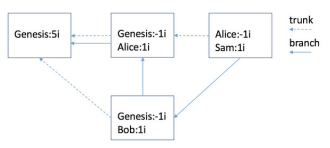
\includegraphics[width=3.0in]{figures/screenshot004.png}
	\caption{confirms successful transaction}
	\label{simulationfigure}
\end{figure}

\begin{figure}[H]
	\centering
	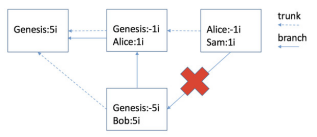
\includegraphics[width=3.0in]{figures/screenshot005.png}
	\caption{confirms the failed transaction, which will cause the Genesis balance to drop to -1}
	\label{simulationfigure}
\end{figure}

\subsubsection{Select tip}
There are two basic concepts in StreamNet, one is the transaction rate, which indicates the number of transactions per time unit. For convenience, we set the time unit to seconds. The other is invisible time, indicating how many time units a transaction has not been seen by other exchanges after attach. Because of some existence, the transaction rate has an important influence on the shape of StreamNet. For example, in Figure 7, when the transaction rate is slow, StreamNet is more like a chain. In the case of block trading in Figure 8, the shape of StreamNet is a star.

\begin{figure}[H]
	\centering
	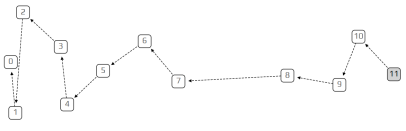
\includegraphics[width=3.0in]{figures/screenshot006.png}
	\caption{StreamNet shape under slow trading}
	\label{simulationfigure}
\end{figure}

\begin{figure}[H]
	\centering
	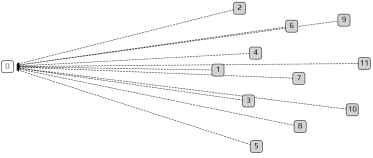
\includegraphics[width=3.0in]{figures/screenshot007.png}
	\caption{StreamNet shape under fast trade}
	\label{simulationfigure}
\end{figure}

One of the most basic tip selection algorithms is to start from Genesis to move the transaction with approval to an equal probability until a tip is selected, as shown in Figure 8. Suppose Alice $\rightarrow$ Sam's transaction wants to select tip, which starts from Genesis transaction. There are two options for this time, one is Genesis $\rightarrow$ Alice, the other is Genesis $\rightarrow$ Bob, the probability of selecting Genesis $\rightarrow$ Alice is 1 /2, while Genesis $\rightarrow$ Bob is 1/2. 

\begin{figure}[H]
	\centering
	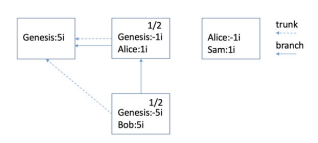
\includegraphics[width=3.0in]{figures/screenshot008.png}
	\caption{Equal Probability Random Walk Algorithm}
	\label{simulationfigure}
\end{figure}

\begin{figure}[H]
	\centering
	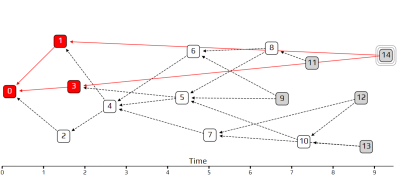
\includegraphics[width=3.0in]{figures/screenshot009.png}
	\caption{lazy transaction example}
	\label{simulationfigure}
\end{figure}

\begin{figure}[H]
	\centering
	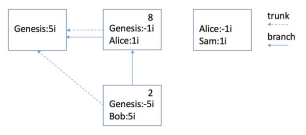
\includegraphics[width=3.0in]{figures/screenshot010.png}
	\caption{Random walk selection tip}
	\label{simulationfigure}
\end{figure}

\begin{figure}[H]
	\centering
	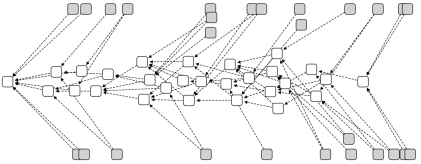
\includegraphics[width=3.0in]{figures/screenshot011.png}
	\caption{super-weight algorithm example diagram}
	\label{simulationfigure}
\end{figure}

The problem with the basic random walk algorithm is that it produces lazy transactions. For example, in Figure 9,transaction 14 is a lazy transaction that causes new transactions to approve older transactions without being penalized. This problem can be solved by using Monte Carlo Random Walk (MCMC). In Figure 10, there is a weight on both transactions, for example, Genesis $\rightarrow$ Alice is 8, and Genesis $\rightarrow$ Bob is 2, then the probability of selecting Genesis $\rightarrow$ Alice is 8/10, and Genesis $\rightarrow$ Bob is 2 /10. The determination of the weight is determined by how many transactions have directly or indirectly approved the transaction. The more approved transactions, the greater the weight. If only deterministic use weights are then a super-weight algorithm, meaning that large-weight transactions are always preferred. The problem with this algorithm is that there are many transactions that can never be confirmed. Figure 11 shows the results of a super-weighted algorithm. For example, if purely using probability weighting, then it is a
super-probability algorithm. The trade-off between the two is represented by a $\alpha$, and it can be considered that the
larger the $\alpha$ is, the smaller the randomness is. The method of specifically using $\alpha$ to calculate the jump probability is expressed in the formula (1). Which represents the weight of the trading node.Where P\_{xy} represents the probability of jumping from x to y. H\_{y} represents the weight of the trading node y.

\begin{equation}
\label{simple_equation}
P_{xy} = \frac{e^{\alpha H_{y}}}{\Sigma_{z:z \rightarrow x}e^{\alpha H_{z}}}
\end{equation}

\subsubsection{Trading Consensus}
There are currently three ways to confirm a transaction in StreamNet:
	\begin{itemize}
		\item The first way is that the common nodes covered by all the previous tips are considered to be fully confirmed; for example, in Figure 12, the nodes referenced or indirectly referenced by tip1 are blue and yellow line covered transactions, while the tip2 reference Or the indirectly referenced node is a yellow line covered transaction. If there are only 1, 2 tips in StreamNet, then the green node is a fully confirmed transaction, while the green node is an unconfirmed transaction.
		\item The second way is that the system sends a Coordinator tip every 1 minute. This tip is called milestone and is attached to StreamNet. All transactions referenced by this Coordinator tip are confirmed.
		\item The third way is to use Monte Carlo Random Walk (MCMC). Call N times to select a tip using the tip selection algorithm. If a trading node is referenced by this tip, its credibility is increased by 1. After M selections have been cited M times, then the credibility is M / N.
  \end{itemize}

\begin{figure}[H]
	\centering
	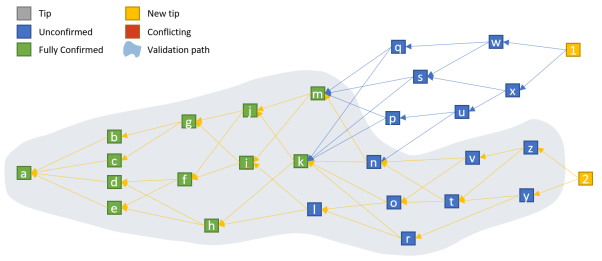
\includegraphics[width=3.0in]{figures/screenshot012.png}
	\caption{fully confirms the node, unconfirmed node [4]}
	\label{simulationfigure}
\end{figure}

